% !Mode:: "TeX:UTF-8"
% !TEX program  = xelatex
\documentclass[a4paper]{article}
\usepackage{amsmath}
\usepackage{amssymb}
\usepackage{ctex}
%\usepackage{braket}
%\usepackage[european]{circuitikz}
\usepackage{multirow}
\usepackage{float}
\usepackage{graphicx}
\usepackage{geometry}
\geometry{left=2.5cm,right=2.5cm,bottom=2.5cm,top=2.5cm}
\title{近代物理实验报告:差热分析}
\author{xy\quad 学号\quad 匡亚明学院}
\date{2019年2月29日}
\begin{document}
\maketitle
\bibliographystyle{unsrt}
%--------main-body------------

\section{引言}
差热分析(DTA)是在程序控制温度下测量物质和参比物之间的温度差与温度(或时间)关系的一种技术。描述这种关系的曲线称为差热曲线或DTA曲线。由于试样和参比物之间的温度差主要取决于试样的温度变化,因此就其本质来说,差热分析是一种主要与焓变测定有关并借此了解物质有关性质的技术。

\section{实验目的}
\begin{enumerate}
\item 掌握差热分析的基本原理及测量方法。
\item 学会差热分析仪的操作,并绘制CuSO$_4\cdot$5H$_2$O等样品的差热图。
\item 掌握差热曲线的处理方法,对实验结果进行分析。
\end{enumerate}

\section{实验仪器}
差热分析仪、计算机、样品。

\section{实验原理}
物质在加热或冷却过程中,当达到特定温度时,会产生物理或化学变化,同时产生吸热和放热的现象,反映了物质系统的焓发生了变化。在升温或降温时发生的相变过程,是一种物理变化,一般来说由固相转变为液相或气相的过程是吸热过程,而其相反的相变过程则为放热过程。在各种化学变化中,失水、还原、分解等反应一般为吸热过程,而水化、氧化和化合等反应则为放热过程。差热分析利用这一特点,通过对温差和相应的特征温度进行分析,可以鉴别物质或研究有关的转化温度、热效应等物理化学性质,由差热图谱的特征还可以用以鉴别样品的种类,计算某些反应的活化能和反应级数等。

在差热分析中,为反映微小的温差变化,用的是温差热电偶。在作差热鉴定时,是将与参比物等量、等粒级的粉末状样品,分放在两个坩埚内,坩埚的底部各与温差热电偶的两个焊接点接触,与两坩埚的等距离等高处,装有测量加热炉温度的测温热电偶,它们的各自两端都分别接人记录仪的回路中在等速升温过程中,温度和时间是线性关系,即升温的速度变化比较稳定,便于准确地确定样品反应变化时的温度。样品在某一升温区没有任何变化,即也不吸热、也不放热,在温差热电偶的两个焊接点上不产生温差,在差热记录图谱上是一条直线,已叫基线。如果在某一温度区间样品产生热效应,在温差热电偶的两个焊接点上就产生了温差,从而在温差热电偶两端就产生热电势差,经过信号放大进入记录仪中推动记录装置偏离基线而移动,反应完了又回到基线。吸热和放热效应所产生的热电势的方向是相反的,所以反映在差热曲线图谱上分别在基线的两侧,这个热电势的大小,除了正比于样品的数量外,还与物质本身的性质有关。

将在实验温区内呈热稳定的已知物质与试样一起放入一个加热系统中,并以线性程序温度对它们加热。如以Al$_2$O$_3$为参比物,它在整个试验温度内不发生任何物理化学变化,因而不产生任何热效应。将参比物和试样分别放在坩埚中然后放入电炉中加热升温。在升温过程中试样如没有热效应则试样与参比物之间的温度差$\Delta T$为零;而试样在某温度下有放热(吸热)效应时,试样温度上升速度加快(减慢),就产生温度差$\Delta T$,把$\Delta T$转变成电信号放大后记录下来,可得差热曲线图。在试样和参比物的比热容、导热系数和质量等相同的理想情况,试样的参比物的温度及它们之间的温度差随时间的变化如图(\ref{fig1})所示。
\begin{figure}[!h]
\centering
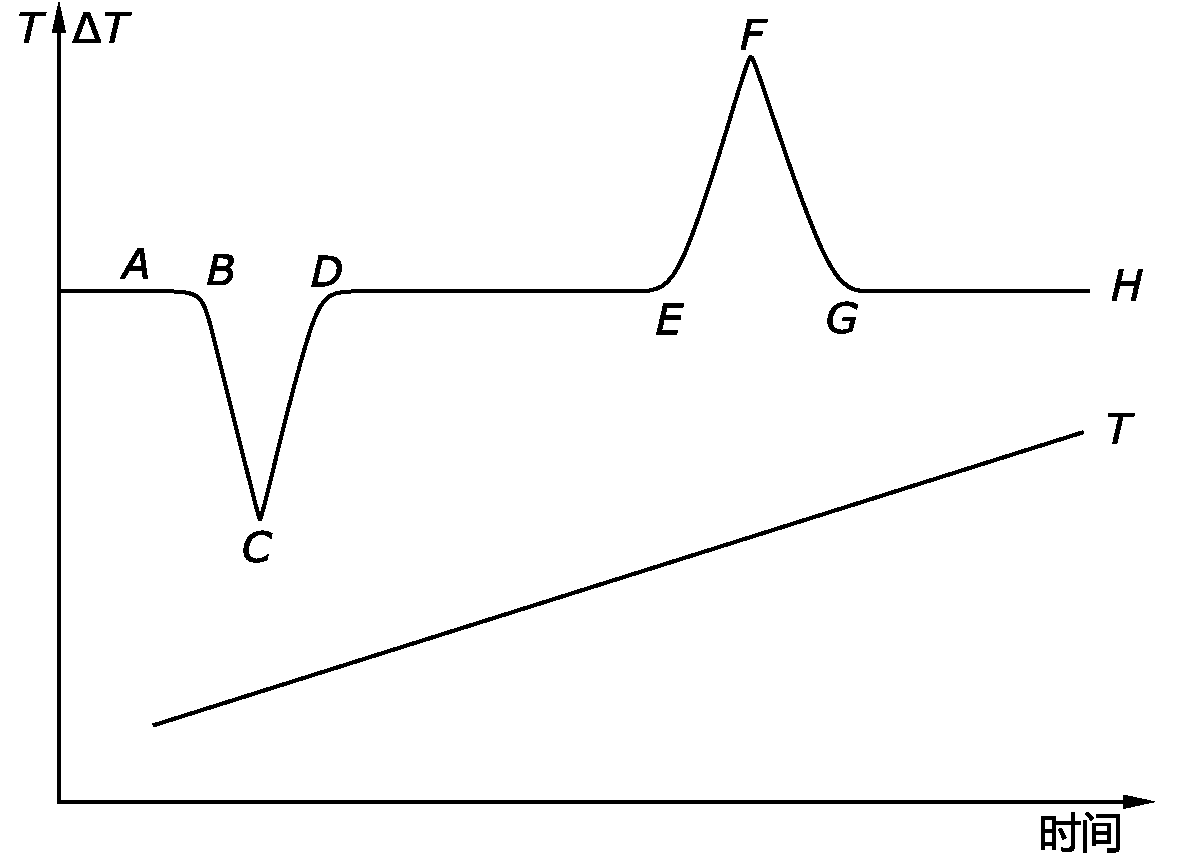
\includegraphics[width=0.6\textwidth]{fig/fig1.pdf}
\caption{差热图}\label{fig1}
\end{figure}

图中参比物的温度始终和程序温度已知,试样温度则随吸热和放热过程的发生而偏离程序温度。当$\Delta T$为零时,图中参比物与试样温度一直,两温度线重合,$\Delta T$曲线则为一条水平基线。

差热图谱中峰的数目表示在测定温度范围内,待测样品发生变化的次数;峰的位置表示发生转化的温度范围;峰的方向指示过程是吸热还是放热;峰的面积反映热效应大小(在相同测定条件)。峰高、峰宽及对称性除与测定条件有关外,往往还与样品变化过程的动力学因素有关。这样从差热图谱中峰的方向和面积可测得变化过程的热效应。

差热峰的面积与过程的热效应成正比,即
\begin{equation}
A = \int_{t_1}^{t_2}\Delta T\text{d}t = KQ_p
\end{equation}
式中m为样品质量;$t_1$、$t_2$分别为峰的起始、终止时刻;$\Delta T$为时间间隔内样品与参比物的温差;$\int_{t_1}^{t_2}$代表面积;K为常数。

\section{实验内容}
\begin{enumerate}
\item 启动计算机,将控制器、加热炉和计算机用相应的接线连接起来。
\item 使用小药匙往小坩埚中装填参比样品和待测样品。
\item 在坩埚架上放置药品,降下炉体。
\item 设定升温速率,启动数据记录软件,开始加热。
\item 记录升温曲线和差热曲线,直至温度升至发生要求的相变且基线变平后,停止记录,保存数据。
\item 打开炉盖,取出坩埚,待炉温降至50$^{\circ}$C以下时,换上另一样品Sn,按上述步骤操作。
\item 处理得到的实验数据。
\end{enumerate}

\section{实验数据}

\section{实验讨论}
\iffalse
\subsection{差热峰的方向与样品吸放热的关系:}
差热峰的方向和两个因素有关,首先,差热分析中是以参比物还是试样为基准来算差值(即$T_S-T_R=\Delta T$还是$T_R-T_S=\Delta T$);其次,发生的反应本身是吸热还是放热的。若以参比物为基准,则放热时$\Delta T<$0,峰向上,吸热时$\Delta T>$0,峰向下;而以试样为基准则是吸热时$\Delta T>$0 ,峰向上,放热时$\Delta T<$0,峰向下。在本次实验中以试样为基准,由于是吸热反应,因此差热峰向上。
\subsection{克服基线漂移,可以采取哪些措施:}
首先,只有当参比物和试样的热性质、质量、密度等完全相同时才能在试样无任何类型能量变化的相应温区内保持DT=0,使基线不发生漂移。参比物的导热系数受比热容、密度、温度和装填方式等多种因素的影响,这些因素的变化均能引起差热曲线基线的偏移。即使同一试样用不同参比物实验,引起的基线偏移也不一样。为减小试样和参比物在热性质上的明显差异造成的基线漂移,可用试样和参比物均匀混合(即稀释试样)后使用的方法来减小。用厚约0.5mm的参比物覆盖试样,也可以减小试样和参比物与环境热交换上的差别,从而提高测量结果的可靠性。

其次,较慢的升温速率,使体系接近平衡条件,基线漂移小。

另外,试样量小,差热曲线出峰明显、分辨率高,基线漂移也小。
\subsection{影响峰高度和峰面积的因素:}
试样的导热系数增加,峰高下降。由于试样装填后的导热能力是由颗粒试样和装填空隙中的气体共同决定的,因此,随着试样容重的改变,装填密度的变化,试样的导热系数也将发生改变。如果粒度改变引起装填空隙减小,而装填空隙中充满的是导热能力较差的空气时,试样的导热能力将随l 变大而增大。从而$\text{DT}_{\text{max}}$峰高下降,峰面积也下降。这种情况常常在粒度增大时发生,而粒度变小产生的是相反的效应。试样装填密度的大小还会影响试样内部的温度梯度。通常,装填密度增加后,会因试样导热能力的增大面使试样内部的温度梯度变小。这时,试样发生变化的温度范围将变窄,并使峰温$T_p$向低温移动,而$\text{DT}_{\text{max}}$,$\text{DT}_{\text{min}}$有可能增加。

对于有气体参加或有气体产物的反应,因粒度改变而使气体的扩散阻力增大时,这不仅阻碍反应进行,而且还会加大气体产物在试样周围的局部分压,导致分解压加大而使分解困难。这时,易使峰高下降、峰宽加大。

惰性稀释剂是为了实现某些目的而掺入试样,覆盖或填于试样底部的物质。当稀释剂的比热容大于试样时,稀释剂的加入还利于试样的比热容保持相对恒定,但使峰高降低。一旦稀释剂使试样的导热系数增加,峰高一般也要下降。

在线性升温时,较快的升温速率通常导致$T_p$向高温移动和峰面积增加,$\text{DT}_{\text{max}}$($\text{DT}_{\text{min}}$)一般也是增加的。这是因为若仅考虑升温速率,试样在单位时间内发生转变或反应的量随升温速率增大而地加,从而使始变速率$\frac{\text{d}H}{\text{d}t}$增加。由于差热曲线从峰返回基线的温度是由时间和试样与参比物间的温度差决定的,所以升温速率增加,曲线返回基线时或热效应结束时的温度均向高温方向移动。
\fi

\section{误差分析}
\iffalse
该实验通过测量样品和参照物的温差随时间的变化,来研究样品的热学性质。实验的误差主要来源于以下几个方面。
\begin{enumerate}
\item 参比物和样品的热性质、质量、密度等并不完全相同导致基线发生漂移。参比物的导热系数受比热容、密度、温度和装填方式等多种因素的影响,这些因素的变化均能引起差热曲线基线的偏移。因此,即使装填时对样品进行小心振动使样品尽量装填紧密,还是不能避免误差的产生。
\item 试样的用量偏大会导致相邻的两个峰发生重叠,在进行近似处理时不可避免的会带来系统误差,因此实验时可减少试样用量,是差热曲线更准确更便于分析处理。
\item 升温速率的影响。升温过快会导致峰变尖锐,图像各点的离散程度变大,不利于数据的处
理,且升温过快会使实验受环境温度的影响变大,容易导致加热器内温度的不均匀。
\item 在拟合过程中,如果把峰值附近的数据点分别拟合,并且对得到的函数进行积分,很容易能得到峰下包围的面积,但是由于第一与第二个峰相互重叠,但是这样算下来的误差比较大,所以采用计算半峰面积再乘以2的方法。这种办法要求差热峰有良好的左右对称性,但从实验数据上来看,差热峰的对称性并不是很好,所以这样处理还是有一定的误差。
\item 热力学平衡温度来源于峰前斜率最大处切线与基线的交点,故基线的选择对结果有一定的影响。
\end{enumerate}
\fi

\section{思考题}
\subsection{差热分析为什么要用参考物?对它有什么要求?}
\subsection{本实验中为什么参考物都置于样品支持器中?}
\subsection{如何辨明反应是吸热还是放热?为什么加热过程中,即使样品没有发生变化,差热曲线仍然会出现较大的漂移?}
\subsection{反应前后差热曲线的基线往往不在一条水平线上,为什么?}
\subsection{为使本实验重复性好,应注意哪些问题?}

\nocite{jiaocai}
\bibliography{ref}
\end{document}